\newtheorem{mydef}{Definición}
\section{BBO: Biogeography-based Optimization Algorithm}


\subsection{Introducción}
\label{sec:meta1_intro}

La Optimización Basada en Biogeografía (BBO) es un algoritmo de optimización inspirada en la biogeografía, que es el estudio de cómo se distribuyen geográficamente las especies biológicas.

Fue propuesto por Dan Simon en 2008 \cite{simon2008biogeography}, como un método para resolver problemas de optimización complejos. 
BBO se basa en la idea de que las soluciones a un problema pueden ser representadas como "hábitats" en un ecosistema, y que la calidad de estas soluciones puede ser evaluada mediante un índice de idoneidad (HSI, por sus siglas en inglés).

Este algoritmo mantiene una población fija de soluciones y las modifica en cada iteración mediante dos operadores principales: migracion y mutación.

\subsubsection{Migración} \label{sec:migration}

Supongamos que tenemos un problema y una población de soluciones candidatas representada como un vector de números enteros. Cada uno de estos números enteros es considerado un SIV (\textit{Suitability Index Variable}).
Las soluciones que son buenas son consideradas habitantes con un HSI alto y las que son malas tienen un HSI bajo. Las soluciones con un HSI alto representan hábitats de muchas especies mientras las soluciones con un HSI bajo representan hábitats de pocas especies. Supongamos dos soluciones $S_1$ y $S_2$ para la explicación:

\begin{itemize}
    \item $S_1$ es considerada una solución con un HSI bajo, representa un hábitat con pocas especies. Su tasa de inmigración $\lambda_1$ va a ser más alta que $\lambda_2$. Su tasa de emigración $\mu_1$ va a ser más baja que $\mu_2$.
    \item $S_2$ es considerada una solución con un HSI alto, representa un hábitat con muchas especies. Su tasa de inmigración $\lambda_2$ va a ser más baja que $\lambda_1$. Su tasa de emigración $\mu_2$ va a ser más alta que $\mu_1$.
\end{itemize}
Se utilizan las tasas de emigración ($\mu$) e inmigración ($\lambda$) de cada solución para compartir información probabilísticamente entre hábitats15. El proceso de modificación funciona así:
\begin{itemize}
    \item La probabilidad de que una solución $H_i$ sea seleccionada para ser modificada es proporcional a su tasa de inmigración $\lambda_i$.
    \item Si la solución $H_i$ es seleccionada para ser modificada, se usa la tasa de emigración $\mu_j$ de las otras soluciones ($j \neq i$) para decidir probabilísticamente cuál de ellas donará un SIV.
    \item Se selecciona un SIV aleatorio de la solución donante $H_j$ y este reemplaza a un SIV aleatorio en la solución receptora $H_i$.
\end{itemize}
La migración en BBO es un proceso adaptativo; se usa para modificar las "islas" (soluciones) existentes 19. Además, como en otros algoritmos basados en población, se incorpora elitismo para retener las mejores soluciones, evitando que sean corrompidas por la inmigración.


\subsubsection{Mutación} \label{sec:mutation}Los eventos aleatorios pueden cambiar drásticamente el HSI de un hábitat. Esto se modela en BBO como la mutación del SIV, y se usan las probabilidades de conteo de especies para determinar las tasas de mutación10. Las probabilidades de las especies se rigen por la Ecuación (2).\\

Cada miembro de la población tiene una probabilidad asignada ($P_s$), la cual hace referencia a la probabilidad que tenía a priori de existir como una solución al problema12. Tanto las soluciones con un HSI muy alto como las soluciones con un HSI muy bajo son igualmente improbables13. Las soluciones con un HSI medio son, en comparación, muy probables.\\

Si una solución $S$ tiene una baja probabilidad $P_s$, es sorprendente que exista y, por lo tanto, es probable que mute a otra solución. Por el contrario, una solución con una probabilidad alta es menos probable que mute. La siguiente fórmula define la tasa de mutación $m$, la cual es inversamente proporcional a la probabilidad de la solución:

$$m(S) = m_{\text{max}} \left( \frac{1 - P_s}{P_{\text{max}}} \right)$$

En esta fórmula, $m_{max}$ es un parámetro definido por el usuario18. Este enfoque tiende a aumentar la diversidad entre la población19. Sin él, las soluciones más probables (HSI medio) tenderían a dominar la población. Este mecanismo hace que las soluciones con HSI bajo sean propensas a mutar (dándoles la oportunidad de mejorar) y que las soluciones con HSI alto también lo sean (dándoles la oportunidad de mejorar aún más).\\

Es importante recalcar que se utiliza un enfoque elitista. Se guardan las mejores soluciones antes de la mutación, de modo que si una mutación de "alto riesgo" arruina el HSI de una buena solución, la original se conserva. Se espera que las soluciones con HSI medio (las más probables) mejoren a través de la migración, por lo que se evita mutarlas (aunque conservan una pequeña probabilidad de mutación).\\

El mecanismo de mutación implementado depende del problema24. Por ejemplo, en el problema de selección de sensores discutido en el artículo, la mutación consiste en reemplazar un sensor (SIV) escogido aleatoriamente por otro sensor generado también aleatoriamente.

\subsection{Definiciones previas}
\label{sec:meta1_algoritmo}

El algoritmo está construido en base a una serie de definiciones preliminares que le dan forma a la estructura del mismo, pasando de un lenguaje
basado en la biología con conceptos como hábitat a un lenguaje computacional. 
A continuación se presentan dichas definiciones:

\begin{mydef}
    Un hábitat es un vector de $m \in \mathbb{N}$ enteros que representa una solución factible al problema.
\end{mydef}

\begin{mydef}
    El índice variable de idoneidad es un entero que es permitido en el hábitat. 
\end{mydef}

\begin{mydef}
    El índice de idoneidad del hábitat $HSI: H \rightarrow \mathbb{R}$ es una medida de la bondad de la solución representada por el hábitat. En los algoritmos de optimización basados en población se denomina fitness.
\end{mydef}

\begin{mydef}
    Un ecosistema $H^{n}$ es un grupo de $n \in \mathbb{N}$ hábitats.
\end{mydef}

\begin{mydef}
    La tasa de inmigración $\lambda: \mathbb{R} \rightarrow \mathbb{R}$ es una función monótona no creciente del HSI.
\end{mydef}

\begin{mydef}
    La tasa de emigración $\mu: \mathbb{R} \rightarrow \mathbb{R}$ es una función monótona no decreciente del HSI.
\end{mydef}

En la práctica, asumimos que $\lambda$ y $\mu$ son funciones lineales con los mismos máximos.

\begin{mydef}
    La modificación del hábitat $\Omega: H^{n} \rightarrow H$ es un operador probabilístico que ajusta el hábitat $H$ basado en el 
    ecosistema $H^{n}$. 
    La probabilidad de que H sea modificado es proporcional a la tasa de inmigración $\lambda$, y la probabilidad de que el origen de 
    la modificación sea el hábitat $H_{j}$ es proporcional a la tasa de emigración $\mu_j$. 
\end{mydef}

    Esta función se puede describir de la siguiente manera:

\begin{mydef}
    Mutación $M: H \rightarrow H$ es un operador probabilístico que modifica de forma aleatoria un hábitat.
\end{mydef}

    Esta función se puede describir de la siguiente manera:

\begin{mydef}
    La función de transición del ecosistema $\psi = (m,n,\lambda,\mu,\Omega,M): H^{n} \rightarrow H^{n}$ es una 
    séxtupula que modifica el ecosistema desde una iteración a la siguiente. \\
    Comienza calculando las tasas de inmigración y emigración para cada hábitat en el ecosistema. Luego la función de modificación del hábitat 
    actúa sobre cada hábitat en el ecosistema, seguido por el cálculo del HSI. Y finalmente, se produce la mutación, seguido del cálculo del HSI 
    para cada hábitat.
\end{mydef}

\begin{mydef}
    El algoritmo $BBO = (\mathcal{I},\psi,\mathcal{T})$ es una tripleta que propone una solución a un problema de optimización, donde:
    \begin{itemize}
        \item $\mathcal{I}: \emptyset \rightarrow {H^{n},HSI^{n}}$ es una función que crea un ecosistema inicial de hábitats y calcula cada HSI correspondiente.
        \item $\psi$ es la función de transición del ecosistema.
        \item$ \mathcal{T}: H^{n} \rightarrow {true,false}$ es un criterio de terminación.
    \end{itemize}
\end{mydef}

\subsection{Algoritmo}

Después de toda una serie de definiciones que transforman conceptos biológicos a un lenguaje computacional, vamos a describir el algoritmo BBO de forma secuencial:

\begin{enumerate}
    \item Inicializamos los parámetros del BBO. 
    \item Inicializamos un conjunto aleatorio de hábitats, donde cada hábitat se corresponde con una solución potencial al problema dado.
    Se trata de la implementación del operador $\mathcal{I}$.
    \item Para cada hábitat, mapeamos el HSI al número de especies, S, la tasa de inmigración $\lambda$ y la tasa de emigración $\mu$.
    \item Utilizamos la inmigración y emigración de forma probabilística para modificar cada hábitat no elitista, y recalculamos cada HSI.
    \item Para cada hábitat, actualizamos la propabilidad de sus especies usando la siguiente ecuación: 
    \[
    \dot{P}_s =
    \begin{cases}
    -(\lambda_s + \mu_s) P_s + \mu_{s+1} P_{s+1}, & \text{si } s = 0, \\[8pt]
    -(\lambda_s + \mu_s) P_s + \lambda_{s-1} P_{s-1} + \mu_{s+1} P_{s+1}, & \text{si } 1 \le s \le S_{\max}-1, \\[8pt]
    -(\lambda_s + \mu_s) P_s + \lambda_{s-1} P_{s-1}, & \text{si } s = S_{\max}.
    \end{cases}
    \]

    A continuación mutamos cada hábitat no elitista basándonos en su probabilidad y recalculamos cada HSI.

    \item Volvemos al paso (3) para la siguiente iteración. Este bucle termina después de cierto número de generaciones previamente definido o después de haber 
    encontrado una solución aceptable para el problema. Esto es la implementación del operador $\mathcal{T}$.

\end{enumerate}



\subsection{Diferencias entre BBO y otros algoritmos de optimización basados en poblaciones}

BBO es un algoritmo de optimización basado en poblaciones que no aplica reproducción o la generación de descendientes, lo que claramente lo diferencia de otros algoritmos como los algoritmos genéticos o estrategias evolutivas.

También se distingue de algoritmos como ACO (Optimización por Colonia de Hormigas) porque este último genera un nuevo conjunto de soluciones en cada iteración, mientras BBO mantiene el conjunto de soluciones de una iteración a la siguiente, basándose en la migración para adaptar probabilísticamente esas soluciones.

Las mayores características las comparte con algoritmos como PSO (Optimización por Enjambre de Partículas) y DE (Evolución Diferencial), ya que estos también mantienen una población fija de soluciones, pero cada solución es capaz de aprender de su entorno y adaptarse con el progreso del algoritmo.
Sin embargo, BBO se diferencia de estos algoritmos en que sus soluciones cambian directamente según la migración desde otras soluciones. Luego, las soluciones de BBO comparten directamente sus atributos con otras soluciones.

\subsection{Implementación}
\label{sec:meta2_implementacion}
Para la implementación del algoritmo de BBO para se ha decidido utilizar \verb|Python 3| por su gran cantidad de librerías y su eficiencia en Jupyter Notebook. Se utilizaron librerías como \verb|Numpy| para cálculos numéricos vectorizados, \verb|Matplotlib.pyplot| para generar las gráficas de los frentes de Pareto, \verb|random| para funciones de aleatoriedad, \verb|copy| para crear clones de las soluciones candidatas y \verb|scipy.special.comb| para el cálculo de coeficientes binomiales necesarios en el proceso de mutación.

El código se organizó en varios componentes en un Jupyter Notebook. En la primera parte del documento se han definido las seis funciones de prueba ($\mathcal{T}_1$ a $\mathcal{T}_6$) especificadas en el paper \cite{zitzler2000comparison}. Cada funcion acepta un vector de solución y devuelve los dos objetivos $f_1$ y $f_2$. El código permite los dos tipos de variables de las funciones de prueba: vectores de números decimales (\verb|float|) para las funciones $\mathcal{T}_1, \mathcal{T}_2, \mathcal{T}_3, \mathcal{T}_4$ y $\mathcal{T}_6$, y la estructura especial de arrays de bits para la función $\mathcal{T}_5$.

Para representar una solución individual, se ha creado la clase \verb|Habitat|. Esta clase guarda los valores de la solución (\verb|sivs|), su valor de fitness (\verb|hsi| - Habitat Suitability Index), y sus tasas de migración ($\lambda$ y $\mu$). Para crear esta clase hay que llamar a su constructor (\verb|__init__|) el cual va a inicializar aleatoriamente los \verb|sivs| según el \verb|problem_type| ('float' o 'bits'), además los decimales están siendo vectorizados en su inicialización mediante \verb|np.random.uniform| para decimales. Por último se ha creado un método \verb|clone()| para duplicar instancias de forma segura usando \verb|copy.deepcopy()|.

La lógica principal del algoritmo BBO se implementó en la función \verb|run_bbo|. Dado que BBO es un algoritmo mono-objetivo, se adaptó para problemas multiobjetivo mediante una estrategia de suma ponderada: el \verb|hsi| de cada hábitat se calculó como $w_1 \cdot f_1 + w_2 \cdot f_2$ para un par de pesos $(w_1, w_2)$ dado. La función sigue el ciclo evolutivo estándar: evaluación del HSI, ordenación de la población, aplicación de elitismo (conservando los \verb|elitism_param| mejores), mapeo lineal de tasas de migración $\lambda$ y $\mu$ basado en el ranking, y los operadores de migración y mutación. Para mejorar la eficiencia, las operaciones de migración para problemas que utilizan decimales se vectorizaron utilizando NumPy, aplicando las operaciones a todos los SIVs simultáneamente mediante máscaras booleanas y \verb|np.where|. La mutación implementada sigue el esquema probabilístico dependiente de la probabilidad de existencia de la especie ($P_s$) descrito en el BBO original. Se precalculó el vector de probabilidades de especie $P_s$ usando una distribución binomial con $S_{max} = \verb|pop_size| - 1$. Luego, para cada hábitat no elitista, se calculó una tasa de mutación individual $m(S)$ usando la fórmula $m(S) = \verb|m_max| \cdot (1 - P_s / P_{max})$ y se aplicó probabilísticamente a cada SIV (vectorizado para \verb|float|, inversión de bit para \verb|bits|). Al final de las generaciones, la función devuelve los valores $(f_1, f_2)$ del mejor hábitat encontrado para los pesos utilizados.

Las simulaciones se realizaron adoptando un enfoque similar al de SOEA (Single-Objective Evolutionary Algorithm) con agregación. Para cada una de las seis funciones de prueba, se ejecutó \verb|run_bbo| un total de 50 veces, cada vez con un par de pesos $(w_1, w_2)$ distinto, obtenidos mediante \verb|np.linspace| para variar $w_1$ de 0 a 1 y calculando $w_2 = 1 - w_1$. Cada una de estas 50 ejecuciones se realizó durante 100 generaciones. Los 50 puntos $(f_1, f_2)$ resultantes (uno por cada par de pesos) se recopilaron y se graficaron como un diagrama de dispersión para visualizar la aproximación del frente de Pareto.

Los parámetros utilizados fueron consistentes en todas las simulaciones: tamaño de población (\verb|POP_SIZE|) de 50, número de generaciones (\verb|GENERATIONS|) de 100, parámetro de elitismo (\verb|ELITISM_PARAM|) de 2, tasa máxima de migración (\verb|MAX_MIGRATION|) de 1.0, y tasa máxima de mutación (\verb|m_max|) de 0.05.


\subsection{Conclusiones}
\label{sec:meta2_Conclusiones}
En este apartado se redactan las conclusiones obtenidas de la implementación del algoritmo BBO adaptado utilizando la estrategia \textit{Single-Objective Evolutionary Algorithm} (SOEA). Esta adaptación se ha realizado utilizando una suma ponderada para poder aplicarlo a los problemas multiobjetivos $\mathcal{T}_1, \ldots, \mathcal{T}_6$ de \cite{zitzler2000comparison}.

En primer lugar, a pesar de que el algoritmo de Optimización Basada en Biogeografía está diseñado para problemas mono-objetivo, se puede adaptar para explorar el frente de Pareto en problemas multiobjetivo. Esta adaptación se ha realizado utilizando una suma ponderada de los pesos $w_1$ y $w_2$, estos pesos van a ir cambiando a lo largo de las 50 ejecuciones. Estos pesos cumplen que $$w_1 + w_2 = 1, \quad w_1 \ge 0, \quad w_2 \ge 0$$\\

Los resultados recogidos en la Figura \ref{fig:resultados_bbo_3x2} demuestran que para la mayoría de funciones, BBO consigue generar un conjunto de soluciones que se aproxima al frente de Pareto. El mayor aprendizaje que hemos obtenido realizando esta práctica se ha obtenido analizando el comportamiento de BBO en las diferentes funciones de prueba: \\
\begin{itemize}
    \item En las funciones $\mathcal{T}_1$ Convexa y $\mathcal{T}_2$ No Convexa el algoritmo no ha tenido muchos problemas. En la función de prueba $\mathcal{T}_1$, este algoritmo generó puntos bastante cercanos al frente óptimo y con una buena distribución. Esto era esperable ya que las sumas ponderadas funcionan bien para frentes convexos. En cuanto a la función $\mathcal{T}_2$ el algoritmo consiguió dibujar la forma cóncava del frente aunque la distribución de puntos no es uniforme y hay menos densidad de soluciones en el centro.
    \item En la función ($\mathcal{T}_3$) sobre el Frente Discreto, se puede apreciar claramente la discontinuidad de esta función. Las soluciones generadas se agrupan en segmentos separados que componen el frente de Pareto. Podemos concluir que el algoritmo puede identificar y converger a regiones óptimas no continuas.
    \item Las funciones $\mathcal{T}_4$ Multimodal, $\mathcal{T}_5$ Deceptiva están diseñadas para representar Frentes Complejos. En la función $\mathcal{T}_4$ es donde se presentan las mayores dificutlades ya que existen pocas soluciones cercanas al frente de Pareto. En cuanto a $\mathcal{T}_5$ ciertas combinaciones de bits alejan la solución del óptimo global. Con la población de 50 y 100 generaciones, podemos concluir basándonos en los resultados de las gráficas que BBO ha convergido a un frente subóptimo. Es probable que se necesiten poblaciones más grandes, más generaciones, o quizás ajustes en los parámetros de migración/mutación para superar este problema.
    \item En la función $\mathcal{T}_6$ para representar un Frente no Uniforme, el algoritmo ha conseguido representar la forma general del frente. Aunque la densidad de los puntos no es uniforme y existen muchas soluciones en los extremos de $f_1$, este es el comportamiento esperado de esta función. Esto se debe a que es menos probable que las operaciones de migración y mutación del algoritmo generen soluciones en las zonas intermedias por el rango estrecho de valores $x_1$ debido a la forma de la función $\sin^6(6\pi x_1)$.
\end{itemize}

\begin{figure}[htbp]
    \centering
    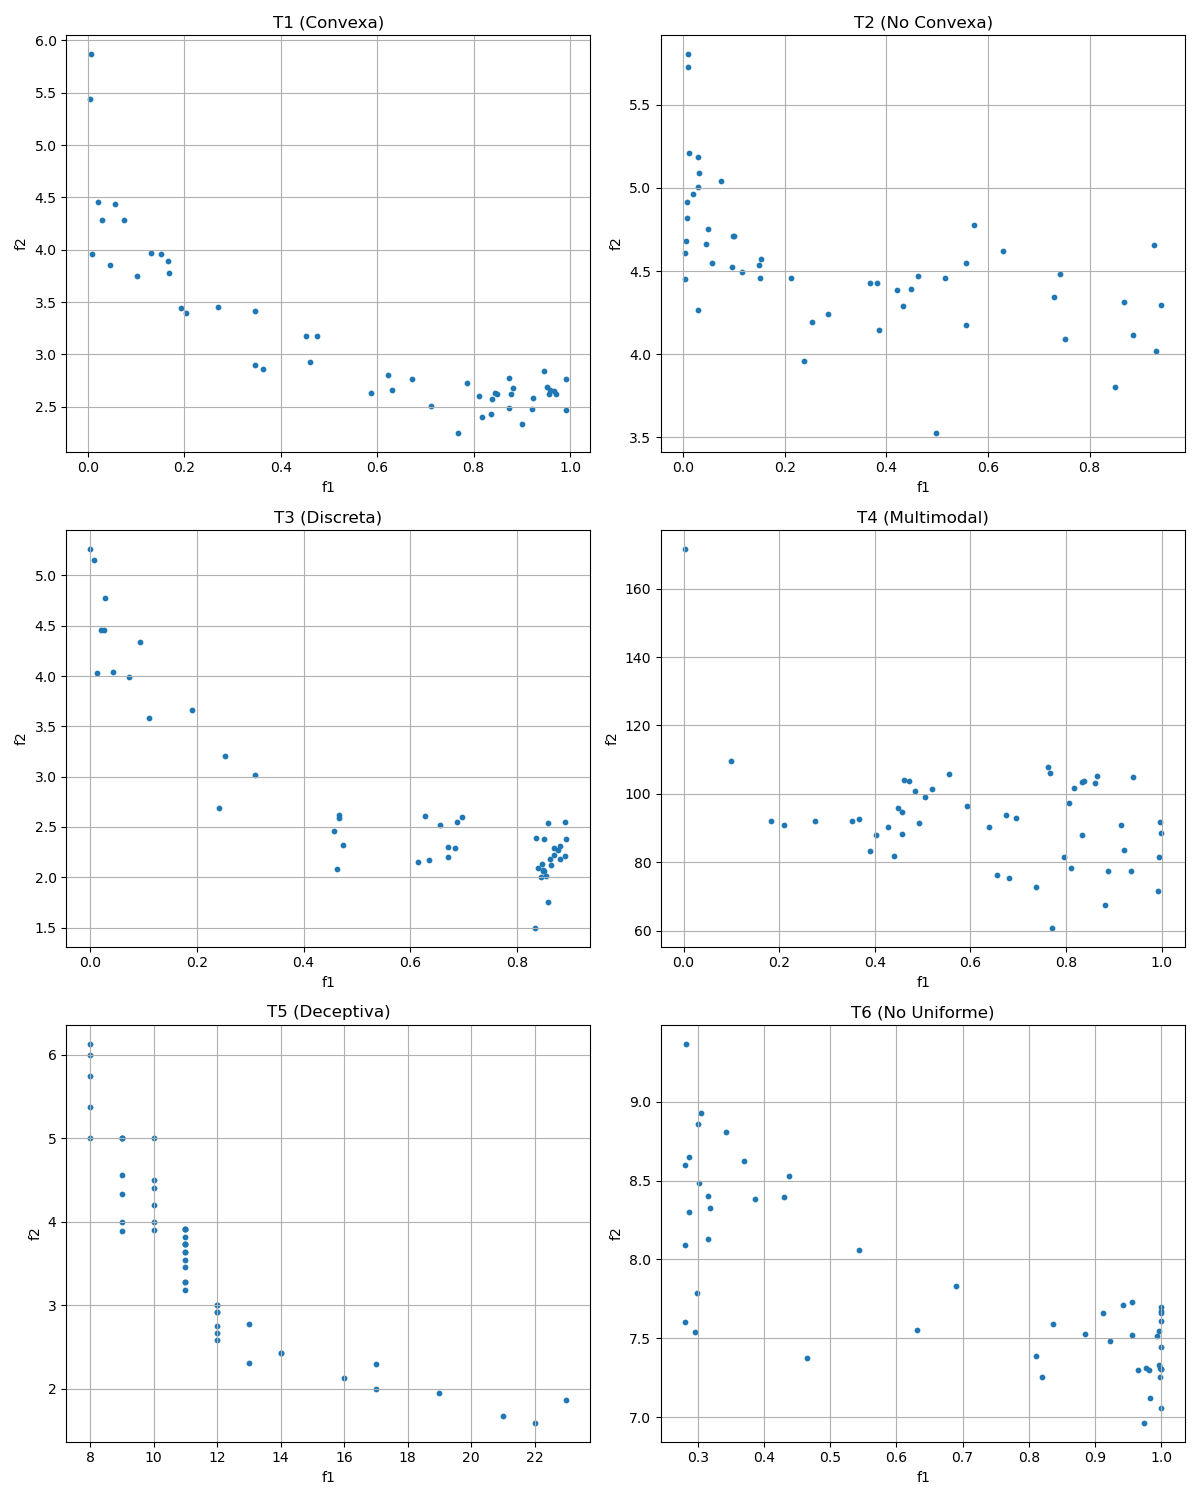
\includegraphics[width=0.9\textwidth]{img/resultados_bbo_3x2.png}
    \caption{Frentes de Pareto aproximados obtenidos por BBO-SOEA para las seis funciones de prueba T1 a T6.}
    \label{fig:resultados_bbo_3x2}
\end{figure}

Mediante la realización de esta práctica, hemos comprendido en profundidad el algoritmo y la analogía que tiene inspirada en la naturaleza y la biología. La implementación de las funciones de prueba ha sido importante para poder ver el rendimiento de este algoritmo en diferentes problemas y poder comprender en qué casos funciona mejor. Ver como BBO se enfrenta a estos problemas \textit{benchmark} nos ha ayudado a comprender y relacionar la teoría vista en clase con la práctica computacional.
